\documentclass{fmbvecto}

\usepackage[spanish]{babel}

\renewcommand{\title}{Ejemplo de solución correcta del taller 2}
\newcommand{\subject}{Cálculo Vectorial}

\renewcommand{\labelenumii}{\theenumii}
\renewcommand{\theenumii}{\theenumi.\arabic{enumii}.}

\NewDocumentCommand{\itemp}{o}{\item (#1 puntos)}

\begin{document}

TODO: Fecha. Jueves, 13 de junio de 2024

\begin{center}
    \textbf{\LARGE \title} \\
    {\large \subject}
\end{center}


Profesor: Jacinto Eloy Puig Portal, \href{mailto:jpuig@uniandes.edu.co}{jpuig@uniandes.edu.co}. \\
Monitor: Federico Melo Barrero, \href{mailto:f.melo@uniandes.edu.co}{f.melo@uniandes.edu.co}.\\

\textbf{\Large Preámbulo}

Las instrucciones referentes a la entrega del taller están escritas en \href{https://bloqueneon.uniandes.edu.co/d2l/home}{Bloque Neón}.

\textbf{Bonos}
\begin{itemize}
  \item Se sumarán 0.5 puntos de bonificación a la nota del taller si su contenido está ordenado y puede leerse con facilidad.
  \item Se sumarán 0.5 puntos de bonificación a la nota del taller si no contiene errores léxicos, gramaticales ni faltas de ortografía.
\end{itemize}
La nota del taller puede exceder el 5.0.

\textbf{Recomendaciones}

No necesita hacer uso de herramientas que le ayuden a hacer matemáticas, ya sean calculadoras, aplicaciones, grandes modelos de lenguaje u otras. Le recomiendo que no lo haga

Recuerde incluir las unidades siempre que trate con magnitudes físicas.

\section{Taller 1}

\begin{problema}[Corrección del taller 1]
    
    (1 punto) Corrija todos los errores que tuvo en el taller 1. Si no tuvo errores, omita este punto.
    
    En este punto simplemente revisaré que hayan corregido sus errores y abordado los comentarios que dejé en su taller. Naturalmente, la corrección debe ser correcta, sobretodo teniendo en cuenta que el solucionario del taller 1 está en Bloque Neón desde el domingo 23 de junio.

\end{problema}

\section{Integrales dobles}

\begin{problema}[Integral doble en región de tipo 3]
    
    (1 punto) Evalúe la integral \[ \int_{1}^{2} \int_{0}^{\ln y} (y-1) \sqrt{1 + \mathrm{e}^{2x}} \: \mathrm{d}x \: \mathrm{d}y. \] No omita ningún paso en su solución.


\vspace{1em}
\tcblower
\textbf{Solución:}

    \subsection{Cambiar el orden de integración}

    Antes de calcular una integral doble, siempre vale la pena inspeccionar la región sobre la que se integra, pues si la región resulta ser de tipo 3, se puede cambiar el orden de integración, lo cual puede facilitar o incluso posibilitar el cálculo de la integral. Para ello, es recomendable hacer un bosquejo de la región. \\
    
    Sea \(D\) la región de integración y \(f(x, y)\) el integrando, de forma que \[ \int_D f = \int_{1}^{2} \int_{0}^{\ln y} (y-1) \sqrt{1 + \mathrm{e}^{2x}} \: \mathrm{d}x \: \mathrm{d}y. \]
    La región \(D\), expresada como región de tipo 2, es el conjunto
    \[D = \{(x, y) | 0 \leq x \leq \ln y \ \land \ 1 \leq y \leq 2\}.\]
    Un bosquejo de la región se muestra en la figura \ref{fig:region-tipo-3}.
    \begin{figure}[H]
        \centering
        % 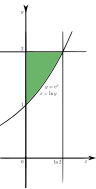
\includegraphics[width=0.5\textwidth]{region-tipo-3.png}
        \caption{Región de integración \(D\).}
        \label{fig:region-tipo-3}
    \end{figure}

    A partir del bosquejo, resulta evidente que \(D\) efectivamente es una región de tipo 3, pues también se puede expresar como región de tipo 1, delimitada por un intervalo numérico en el eje \(x\) y por curvas continuas en el eje \(y\). Se expresa la curva \(x = \ln y\) como \(y = \mathrm{e}^x\), de forma que \(D\) se puede expresar como
    \[D = \{(x, y) | 0 \leq x \leq \ln 2 \ \land \ \mathrm{e}^x \leq y \leq 2\}.\]
    Por lo tanto, la integral se puede reescribir como
    \[ \int_D f = \int_{0}^{\ln 2} \int_{\mathrm{e}^x}^{2} (y-1) \sqrt{1 + \mathrm{e}^{2x}} \: \mathrm{d}y \: \mathrm{d}x. \]

    A partir del proceso anterior, se tienen dos formas de expresar la misma integral. Ahora, se debe ponderar cuál forma es la más conveniente para calcular la integral. En la primera forma, la integral interna es
    \[ \int_{0}^{\ln y} \sqrt{1 + \mathrm{e}^{2x}} \: \mathrm{d}x, \]
    mientras que en la segunda forma, la integral interna es
    \[ \int_{\mathrm{e}^x}^{2} (y-1) \: \mathrm{d}y. \]
    Resulta evidente que es mucho más sencillo calcular la integral en la segunda forma.

    \subsection{Calcular la integral doble}

    Con eso en mente, se procede a calcular la integral.
    \begin{align*}
        \int_D f &= \int_{0}^{\ln 2} \int_{\mathrm{e}^x}^{2} (y-1) \sqrt{1 + \mathrm{e}^{2x}} \: \mathrm{d}y \: \mathrm{d}x \\
        &= \int_{0}^{\ln 2} \sqrt{1 + \mathrm{e}^{2x}} \left( \int_{\mathrm{e}^x}^{2} (y-1) \: \mathrm{d}y \right) \mathrm{d}x \\
        &= \int_{0}^{\ln 2} \sqrt{1 + \mathrm{e}^{2x}} \left( \int_{\mathrm{e}^x}^{2} y \: \mathrm{d}y - \int_{\mathrm{e}^x}^{2} 1 \: \mathrm{d}y \right) \mathrm{d}x \\
        &= \int_{0}^{\ln 2} \sqrt{1 + \mathrm{e}^{2x}} \left( \left. \frac{y^2}{2} \right\vert_{\mathrm{e}^x}^{2} -  1(2 - \mathrm{e}^x) \right) \mathrm{d}x \\
        &= \int_{0}^{\ln 2} \sqrt{1 + \mathrm{e}^{2x}} \left( \frac{2^2}{2} - \frac{(\mathrm{e}^x)^2}{2} - 2 + \mathrm{e}^x \right) \mathrm{d}x \\
        &= \int_{0}^{\ln 2} \sqrt{1 + \mathrm{e}^{2x}} \left( 2 - \frac{\mathrm{e}^{2x}}{2} - 2 + \mathrm{e}^x \right) \mathrm{d}x \\
        &= \int_{0}^{\ln 2} \sqrt{1 + \mathrm{e}^{2x}} \left( \mathrm{e}^x - \frac{\mathrm{e}^{2x}}{2}\right) \mathrm{d}x \\
        &= \int_{0}^{\ln 2} \mathrm{e}^x \sqrt{1 + \mathrm{e}^{2x}} - \frac{\mathrm{e}^{2x}}{2} \sqrt{1 + \mathrm{e}^{2x}} \mathrm{d}x \\
        &= \int_{0}^{\ln 2} \mathrm{e}^x \sqrt{1 + \mathrm{e}^{2x}} \: \mathrm{d}x  - \int_{0}^{\ln 2} \frac{\mathrm{e}^{2x}}{2} \sqrt{1 + \mathrm{e}^{2x}} \: \mathrm{d}x \\
        &= I_1  - I_2.
    \end{align*}

    \subsection{Calcular la integral \(I_1\)}

    Para evaluar \(I_1\) tuve que utilizar tres técnicas de integración: primero, utilizo sustitución simple; luego, sustitución trigonométrica; por último, integración por partes. Además, para reemplazar los valores, me ayudo de un poco de trigonometría. Posiblemente exista un método más elegante o breve para evaluar esta integral, sin embargo, presento este, que utiliza técnicas básicas que vieron en el curso de Cálculo Integral. \\
    
    Como primer paso para evaluar \(I_1\), se realiza el cambio de variable \(u = \mathrm{e}^{x}\), de forma que \(\mathrm{d}u = \mathrm{e}^{x} \: \mathrm{d}x\). Se deben modificar también los límites de integración: para el límite superior, se tiene \(u = \mathrm{e}^{\ln 2} = 2\); para el límite inferior, se tiene \(u = \mathrm{e}^{0} = 1\). Por lo tanto,
    \[ I_1 = \int_{0}^{\ln 2} \mathrm{e}^x \sqrt{1 + \mathrm{e}^{2x}} \: \mathrm{d}x = \int_{1}^{2} \sqrt{1 + u^2} \: \mathrm{d}u. \]
    Lo anterior es una integral de una variable con una suma de cuadrados dentro de un radical. Ergo, es natural usar sustitución trigonométrica para resolverla. Se realiza el cambio de variable \(u = \tan \theta\), de forma que \(\mathrm{d}u = \sec^2 \theta \: \mathrm{d}\theta\). Se deben modificar también los límites de integración: para el límite inferior, se tiene \(\theta = \arctan 1 = \frac{\pi}{4}\); para el límite superior, se tiene \(\theta = \arctan 2\). Por lo tanto,
    \begin{align*}
        I_1 &= \int_{1}^{2} \sqrt{1 + u^2} \: \mathrm{d}u \\
        &= \int_{\frac{\pi}{4}}^{\arctan 2} \sqrt{1 + \tan^2 \theta} \sec^2 \theta \: \mathrm{d}\theta \\
        &= \int_{\frac{\pi}{4}}^{\arctan 2} \sqrt{\sec^2 \theta} \sec^2 \theta \: \mathrm{d}\theta \\
        &= \int_{\frac{\pi}{4}}^{\arctan 2} \sec^3 \theta \: \mathrm{d}\theta.
    \end{align*}
    Para evaluar la integral de secante cúbica, una opción es expresarla como el producto \(\sec^3 \theta = \sec^2 \theta \sec \theta\) y usar integración por partes. En pos de la simplicidad, se evaluará como integral indefinida. Recuérdese la fórmula de integración por partes,
    \[ \int u \: \mathrm{d}v = uv - \int v \: \mathrm{d}u. \]
    Se elige \(u = \sec \theta\) y \(\mathrm{d}v = \sec^2 \theta \: \mathrm{d}\theta\), pensando en sacar provecho de que \(\der[][\theta] \tan \theta = \sec^2 \theta\). Se tiene entonces que \(\mathrm{d}u = \sec \theta \tan \theta \: \mathrm{d}\theta\) y \(v = \tan \theta\). Por lo tanto,
    \begin{align*}
        \int \sec^3 \theta \: \mathrm{d}\theta &= \sec \theta \tan \theta  - \int \tan \theta \sec \theta \tan \theta \: \mathrm{d}\theta \\
        &=  \sec \theta \tan \theta  - \int \sec \theta \tan^2 \theta \: \mathrm{d}\theta \\
        &=  \sec \theta \tan \theta  - \int \sec \theta (\sec^2 \theta - 1)\: \mathrm{d}\theta \\
        &=  \sec \theta \tan \theta  - \int \sec^3 \theta - \sec \theta \: \mathrm{d}\theta \\
        &=  \sec \theta \tan \theta  - \int \sec^3 \theta \: \mathrm{d}\theta + \int \sec \theta \: \mathrm{d}\theta \\
        2 \int \sec^3 \theta \: \mathrm{d}\theta &= \sec \theta \tan \theta + \int \sec \theta \: \mathrm{d}\theta \\
        \int \sec^3 \theta \: \mathrm{d}\theta &= \frac{1}{2} \sec \theta \tan \theta + \frac{1}{2} \ln |\sec \theta + \tan \theta| + C.
    \end{align*}
    En ese último paso, la integral de \(\sec \theta\) es conocida. Si no la recuerda, se calcula multiplicando el integrando por \(\frac{\sec \theta + \tan \theta}{\sec \theta + \tan \theta}\) para obtener una integral de la forma \(\indint{\frac{f'(x)}{f(x)}}[x] = \ln \abs{f(x)} + C\). Con eso, se tiene el valor de la integral de secante cúbico, que se puede reemplazar en la integral \(I_1\) para obtener su valor.
    \begin{align*}
        I_1 =& \int_{\frac{\pi}{4}}^{\arctan 2} \sec^3 \theta \: \mathrm{d}\theta \\
        =& \frac{1}{2} \sec \theta \tan \theta + \frac{1}{2} \ln |\sec \theta + \tan \theta| \Bigg\vert_{\frac{\pi}{4}}^{\arctan 2} \\
        =& \frac{1}{2} \sec (\arctan 2) \tan (\arctan 2) + \frac{1}{2} \ln |\sec (\arctan 2) + \tan( \arctan 2)| \\ &- \frac{1}{2} \sec \frac{\pi}{4} \tan \frac{\pi}{4} - \frac{1}{2} \ln \left|\sec \frac{\pi}{4} + \tan \frac{\pi}{4}\right|
    \end{align*}
    Para calcular los valores, note que, por trigonometría:
    \begin{itemize}
        \item \(\sec \frac{\pi}{4} = \sqrt{2}\),
        \item \(\tan \frac{\pi}{4} = 1\),
        \item \(\sec (\arctan 2) = \sqrt{1 + 2^2} = \sqrt{5}\),
        \item \(\tan (\arctan 2) = 2\).
    \end{itemize}
    Si no lo recuerda, puede hacer dos cosas: primero, dibujar un triángulo rectángulo con ángulo de \(\frac{\pi}{4}\) radianes y catetos de longitud 1, para percatarse de que la hipotenusa tendrá longitud \(\sqrt{2}\); segundo, convencerse de que \(\tan (\arctan x) = x\) y \(\sec (\arctan x) = \sqrt{1 + x^2}\), lo cual se puede deducir manipulando cualquier triángulo rectángulo. \\
    
    Reemplazando los valores anteriores en la expresión para \(I_1\), se tiene que
    \begin{align*}
        I_1 =& \frac{1}{2} \sqrt{5} \cdot 2 + \frac{1}{2} \ln |\sqrt{5} + 2| - \frac{1}{2} \sqrt{2} \cdot 1 - \frac{1}{2} \ln |\sqrt{2} + 1| \\
        =& \sqrt{5} + \frac{\ln(\sqrt{5} + 2)}{2}  - \frac{\sqrt{2}}{2}  - \frac{\ln(\sqrt{2} + 1)}{2}.
    \end{align*}

    \subsection{Calcular la integral \(I_2\)}

    Para evaluar \(I_2\), se realiza un cambio de variable similar al anterior, \(u = \mathrm{e}^{2x}\). Así, \(\mathrm{d}u = 2 \mathrm{e}^{2x} \: \mathrm{d}x\), y los límites de integración se modifican de la siguiente manera: para el límite superior, se tiene \(u = \mathrm{e}^{2 \ln 2} = 4\); para el límite inferior, se tiene \(u = \mathrm{e}^{2 \cdot 0} = 1\). Por lo tanto,
    \[ I_2 = \int_{0}^{\ln 2} \frac{\mathrm{e}^{2x}}{2} \sqrt{1 + \mathrm{e}^{2x}} \: \mathrm{d}x = \frac{1}{4} \int_{1}^{4} \sqrt{1 + u} \: \mathrm{d}u. \]
    Aunque esta integral se asemeja superficialmente a la anterior, note que la expresión dentro del radicando es una función lineal. Esto hace que integrarla sea muchísimo más fácil. Basta con la sustitución \(v = 1 + u\), de forma que \(\mathrm{d}v = \mathrm{d}u\). Cambiar los límites de integración es trivial: para el límite inferior, se tiene \(v = 1 + 1 = 2\); para el límite superior, se tiene \(v = 1 + 4 = 5\). Así pues,
    \begin{align*}
        I_2 &= \frac{1}{4} \int_{1}^{4} \sqrt{1 + u} \: \mathrm{d}u \\
        &= \frac{1}{4} \int_{2}^{5} \sqrt{v} \: \mathrm{d}v \\
        &= \frac{1}{4} \left. \frac{2}{3} v^{3/2} \right\vert_{2}^{5} \\
        &= \frac{1}{6} \left( 5^{3/2} - 2^{3/2} \right) \\
        &= \frac{5 \sqrt{5} - 2 \sqrt{2}}{6}.
    \end{align*}

    \subsection{Concluir}

    Finalmente, se reemplazan los valores de \(I_1\) e \(I_2\) en la expresión para la integral original, \(I_1 - I_2\), para obtener el valor de la integral original.
    \begin{align*}
        \int_D f &= I_1 - I_2 \\
        &= \sqrt{5} + \frac{\ln(\sqrt{5} + 2)}{2}  - \frac{\sqrt{2}}{2}  - \frac{\ln(\sqrt{2} + 1)}{2} - \frac{5 \sqrt{5} - 2 \sqrt{2}}{6}.
    \end{align*}
\end{problema}

\end{document}
